\documentclass[12pt]{article}


\usepackage[numbers]{natbib}
\usepackage{graphicx} 
\usepackage{graphics}
\usepackage{amssymb, amsmath, amsthm} 
\usepackage{fontenc} 
\usepackage{amscd,latexsym,amsfonts,amstext,amsbsy}
\usepackage{euscript} 
\usepackage{enumerate} 
\usepackage{color}  
\usepackage{physics}
\usepackage[latin1]{inputenc}
\usepackage{tikz}
\usepackage{mathrsfs}
\usetikzlibrary{shapes,arrows}
\usepackage{multicol}
\usepackage{comment}
\usepackage{color,soul}
\usepackage{combelow}
\bibliographystyle{apa}



\textwidth = 16 cm
\textheight = 24 cm
\oddsidemargin = 0.0 cm
\evensidemargin = 0.0 cm
\topmargin = -2 cm
\parskip = 0.2in
\parindent = 0.0in


\newtheorem{theorem}{Theorem}
\newtheorem{problem}[theorem]{Problem}
\newtheorem{exercise}[theorem]{Exercise}
\newtheorem{corollary}[theorem]{Corollary}
\newtheorem{lemma}[theorem]{Lemma}
\newtheorem{proposition}[theorem]{Proposition}
\newtheorem{proporties}[theorem]{Proporties}
\newtheorem{definition}[theorem]{Definition}
\newtheorem{definitions}[theorem]{Definitions}
\newtheorem{example}[theorem]{Example}
\newtheorem{remark}[theorem]{Remark}

 


\begin{document}
\textbf{Thoughts} \\
\today \\

We include illicit fentanyl use in the class of heroin users, because of the potency of the drug, which is what those addicted to prescription opioids seek--lower cost and a better high. In addition, a portion of those who overdose from the very powerful drug fentanyl are individuals who are using heroin that is laced with it; therefore, the use of fentanyl is oftentimes intertwined with the use of heroin. 


\textcolor{red}{Confusion: someone prescribed fentanyl will be put in P, but then we are assuming since they are only administered the drug in the hospital (source?) that they will not become addicted and that it would require an illicit source outside the hospital to become addicted? %(which would make sense to put in heroin class). 
So even though they are in P, they can't move to A (although we have that pathway and assume everyone in P is homogeneous?). \\ \\
Wasn't able to find data on *illicit* fentanyl users only, such as number of them. Could we include fentanyl overdoses from addicted class instead of heroin class, since the data sorts out which one was the cause anyways? We could add prescription overdose deaths (which probably don't include fentanyl since not prescribed outside hospital) + fentanyl overdose deaths?}



1. Susceptibles ($S$): This portion of the population consists of individuals who are not taking prescription opioids of any kind, nor are using heroin. \\ \\
2. Prescription opioid users ($P$): This class of individuals consists of individuals who are prescribed opioids by a health care provider and take the opioids at a level that is not considered addicted. We note that individuals in this class could be misusing prescription opioids, but not at the level of addiction.  \\ \\
3. Opioid addicts ($A$): This group of individuals are addicted to opioids or are dependent on opioids, but not using heroin or fentanyl. (Although the opioid class of drug includes heroin and fentanyl, here we will take opioids to mean non-heroin and non-fentanyl.) \textcolor{red}{we assume very few, if any, individuals addicted to opioids outside or prescription opioids, but even if they are, they are probably are taking prescription opioids anyways, so this is our reasoning for taking those with pain reliever use disorder as initial condition because already includes those with other non-prescription opioid addiction...may change because not using NSDUH info anymore} \\ \\
4. Heroin users ($H$): This class is composed of individuals who are addicted to heroin or fentanyl. We note that individuals in this class could be using other drugs or are addicted to opioids in addition to heroin or fentanyl, but they are at least addicted to one of these drugs. \\ \\
5. Individuals in treatment/rehabilitation ($R$): This class consists of individuals undergoing treatment for their addiction to opioids and/or heroin, or have been in treatment in the past and are currently not taking opioids, heroin, or fentanyl.

%Still need: susceptibles becoming heroin users, prescription opioid users becoming heroin users, opioid addicts becoming heroin users, prescription opioid users successfully finishing prescription, susceptibles becoming addicted to opioids, prescription opioid users becoming addicted to opioids, ...+more 

For Tennessee, the \textbf{total number of individuals taking prescription opioids} for pain [1]: \\
2013: 1,845,144 \\
2014: 1,824,342 \\
2015: 1,819,581 \\
2016: 1,761,363 \\
2017: 1,636,374 

\textbf{Treatment admissions for prescription opioids} as primary substance of abuse in Tennessee [3] \\ %can get "new arrivals to R" from this info, apparently: integrate dR/dt over time frame interested in (t_1 to t_2) and on RHS, integrate \zeta*A+\nu*H (or can break into two integrals on the RHS), and can get new arrivals; don't have to worry about double counting or people cycling \\
2014: 4,145\\
2015: 4,085 \\
2016: 3,911 \\
\textcolor{red}{We assume that if one were using heroin in addition to prescription opioids, their heroin problem would be the primary reason for going to treatment?}

\textbf{Treatment admissions for heroin} as primary substance of abuse in Tennessee [3]:  \\
2014: 538 \\
2015: 826 \\
2016: 1,184 \\
These numbers do not include fentanyl users explicitly, but we are under the assumption that those who take fentanyl are a subset of those who use heroin, and therefore, would mostly be included in these numbers. We admit the values may be slightly too low, for the cases of individuals who do go to treatment with the primary substance of abuse being fentanyl, but there is not data available for those numbers currently. 

We use data on the number of prescription opioid overdose deaths which include natural, semi-synthetic, and synthetic opioids; however, we subtract out the number of fentanyl overdoses (fentanyl is classified as a synthetic prescription opioid), since those overdoses are counted for in their own category. This results in the following  \textbf{total number of prescription opioid overdose deaths} [2]: \\
2013:(637-53=) 584 \\
2014: (697-69=) 628 \\
2015: (848-169=) 679 \\
2016: (1,009-294=) 715  

We add together the heroin and fentanyl overdoses from the years 2013-2016 for the state of Tennessee. The \textbf{total number of heroin and fentanyl overdoses} for these four years are: \\
2013: (63+53=) 116 \\
2014: (147+69=) 216 \\
2015: (205+169=) 374 \\
2016: (260+294=) 554 [2]. 

%Can use overdose data of heroin compared to number of heroin addicts in order to get a scaling, and then be able to determine number of fentanyl addicts based on the number of fentanyl overdoses. But for now, going with subset argument, that heroin users includes fentanyl users. 

The \textbf{total number of deaths, excluding overdoses} for individuals in Tennessee (took total deaths and subtracted out overdose deaths for the respective years) [6,7]: \\
2013: (63,199-584-116=) 62,499 out of an estimated total population of 6490795 \\
2014: (64,559-628-216=) 63,715 out of an estimated total population of 6540007 \\
2015: (66,329-679-374=) 65,276 out of an estimated total population of 6590726 \\
2016: (67,924-715-554=) 66,655 out of an estimated total population of 6649404 \\


The following are the \textbf{number of individuals initially in each class} for Tennessee: \\
Susceptibles: \\
Prescription opioid users, 2015: 1,819,581 [1] \\
\textit{Opioid addicts: need to find}  \\ %NSDUH stat was counting misusers 
Heroin/fentanyl addicts, 2015/2016 average for ``Past Year Heroin Use": 14,000 [4] \\
\textit{Recovering addicts: won't be able to find because we do not know the total of individuals total that have been in treatment ever in the past for our time frame}  

The number of heroin users do not include fentanyl users explicitly, but we are under the assumption that those who take fentanyl are a subset of those who use heroin, and therefore, would mostly be included in these numbers. We admit the values may be slightly too low, for the cases of individuals who do heroin and not fentanyl, but we have not been able to find data for fentanyl addicts only currently and we are under the assumption that it would be a negligible population that does fentanyl without heroin. \\

Our ordinary differential equation model \textbf{(removing delta pathway)}: 
\[\dv{S}{t} = -\alpha S - \beta_{A} SA  -\beta_{P} SP- \theta_{1} SH +\epsilon P +\mu (P+R) + (\mu+\mu_{A})A + (\mu+\mu_{H}) H \quad (1)\] 
\[\dv{P}{t} = \alpha S - \epsilon P  - \gamma P - \theta_{2}PH- \mu P    \quad(2)\]
\[\dv{A}{t} = \gamma P + \sigma_{A} R +\beta_{A} SA  +\beta_{P} SP -\zeta A - \theta_{3}AH-(\mu + \mu_{A})A   \quad (3)\]
\[\dv{H}{t} = \theta_{1}SH+\theta_{2}PH+\theta_{3}AH + \sigma_{H}R-\nu H-(\mu+\mu_{H})H  \quad (4)\]
\[\dv{R}{t} = \zeta A +\nu H -\sigma_{A}R-\sigma_{H}R -\mu R\quad(5).\]



\vspace{-1cm}

\begin{figure}[!htb]
\hspace{-.8cm}
\begin{minipage}{.6\textwidth}
\centering
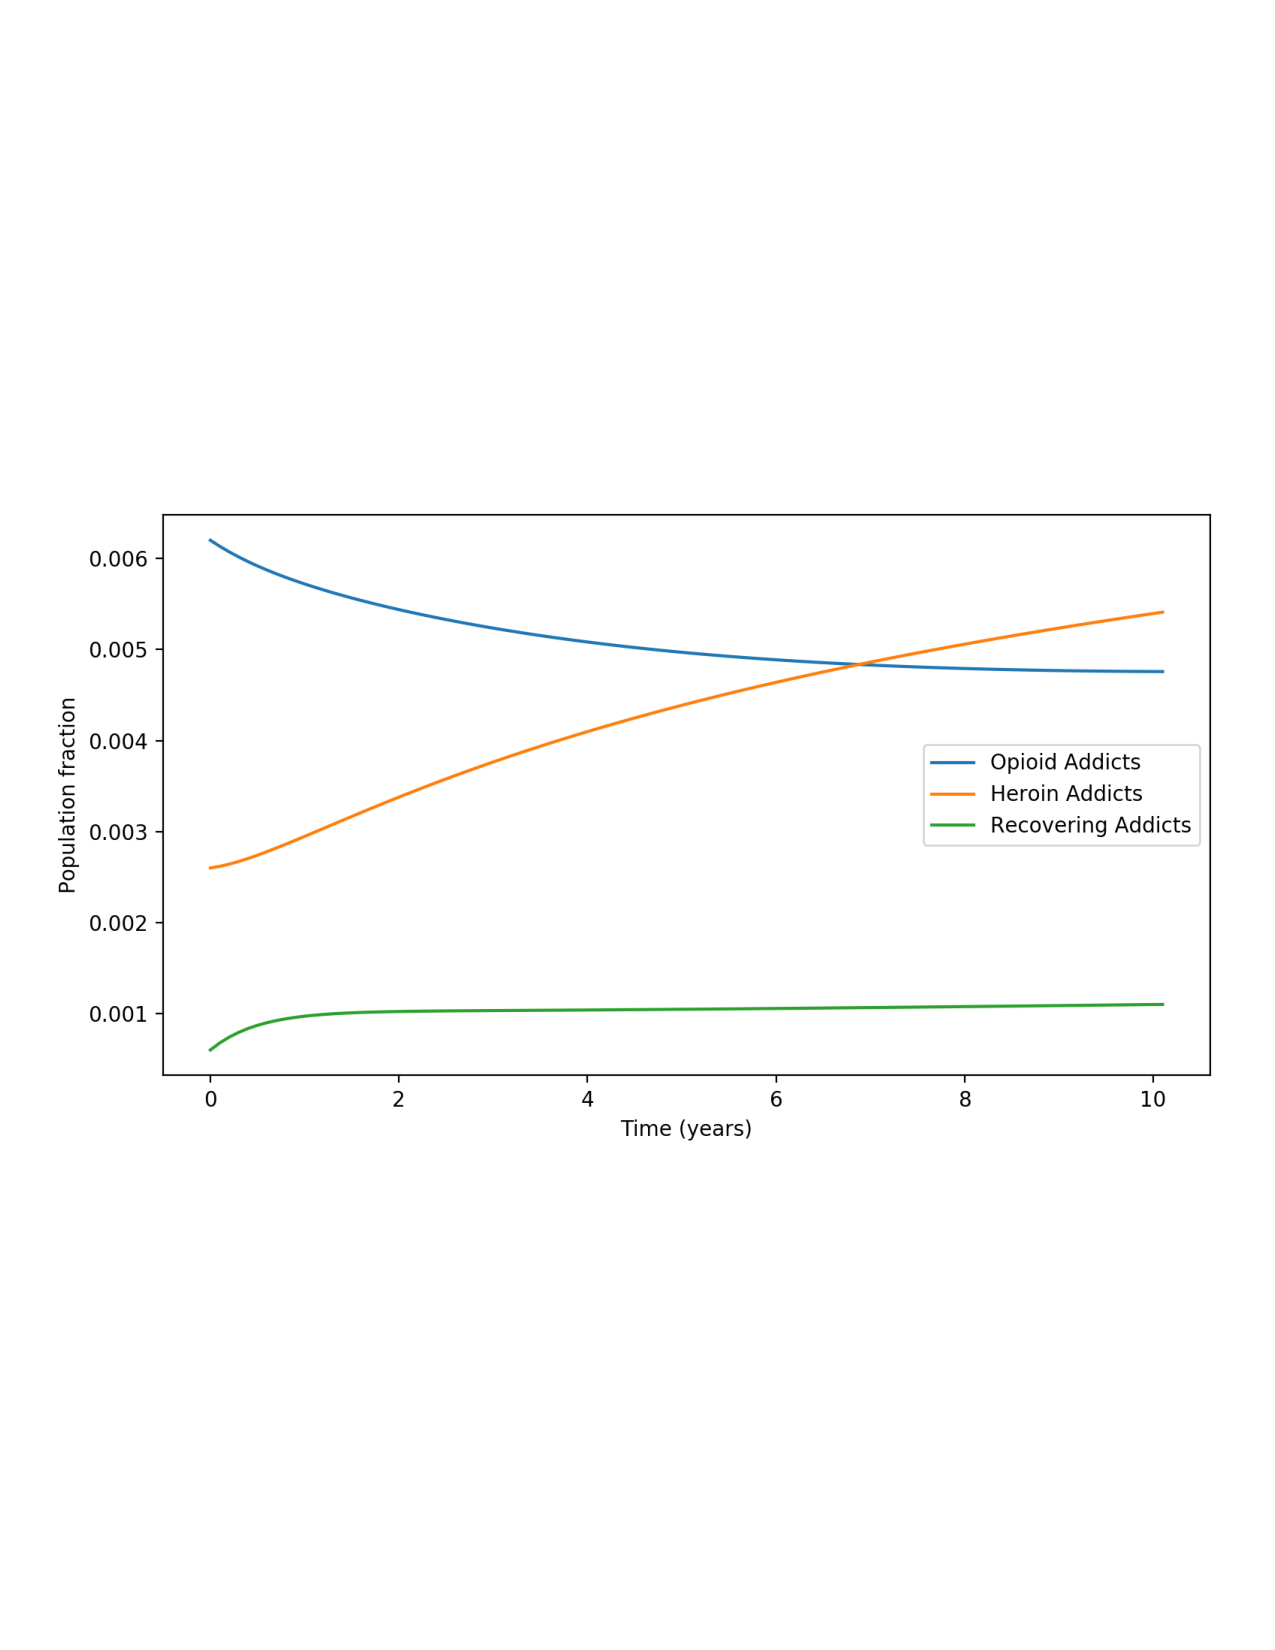
\includegraphics[width=.2\linewidth, height=0.26\textheight]{plot_with_delta_separate}
\vspace{-.4cm}
\caption{Model including delta}
\end{minipage}
\hspace{-1.3cm}
\vspace{.5cm}
\begin{minipage}{.6\textwidth}
\centering
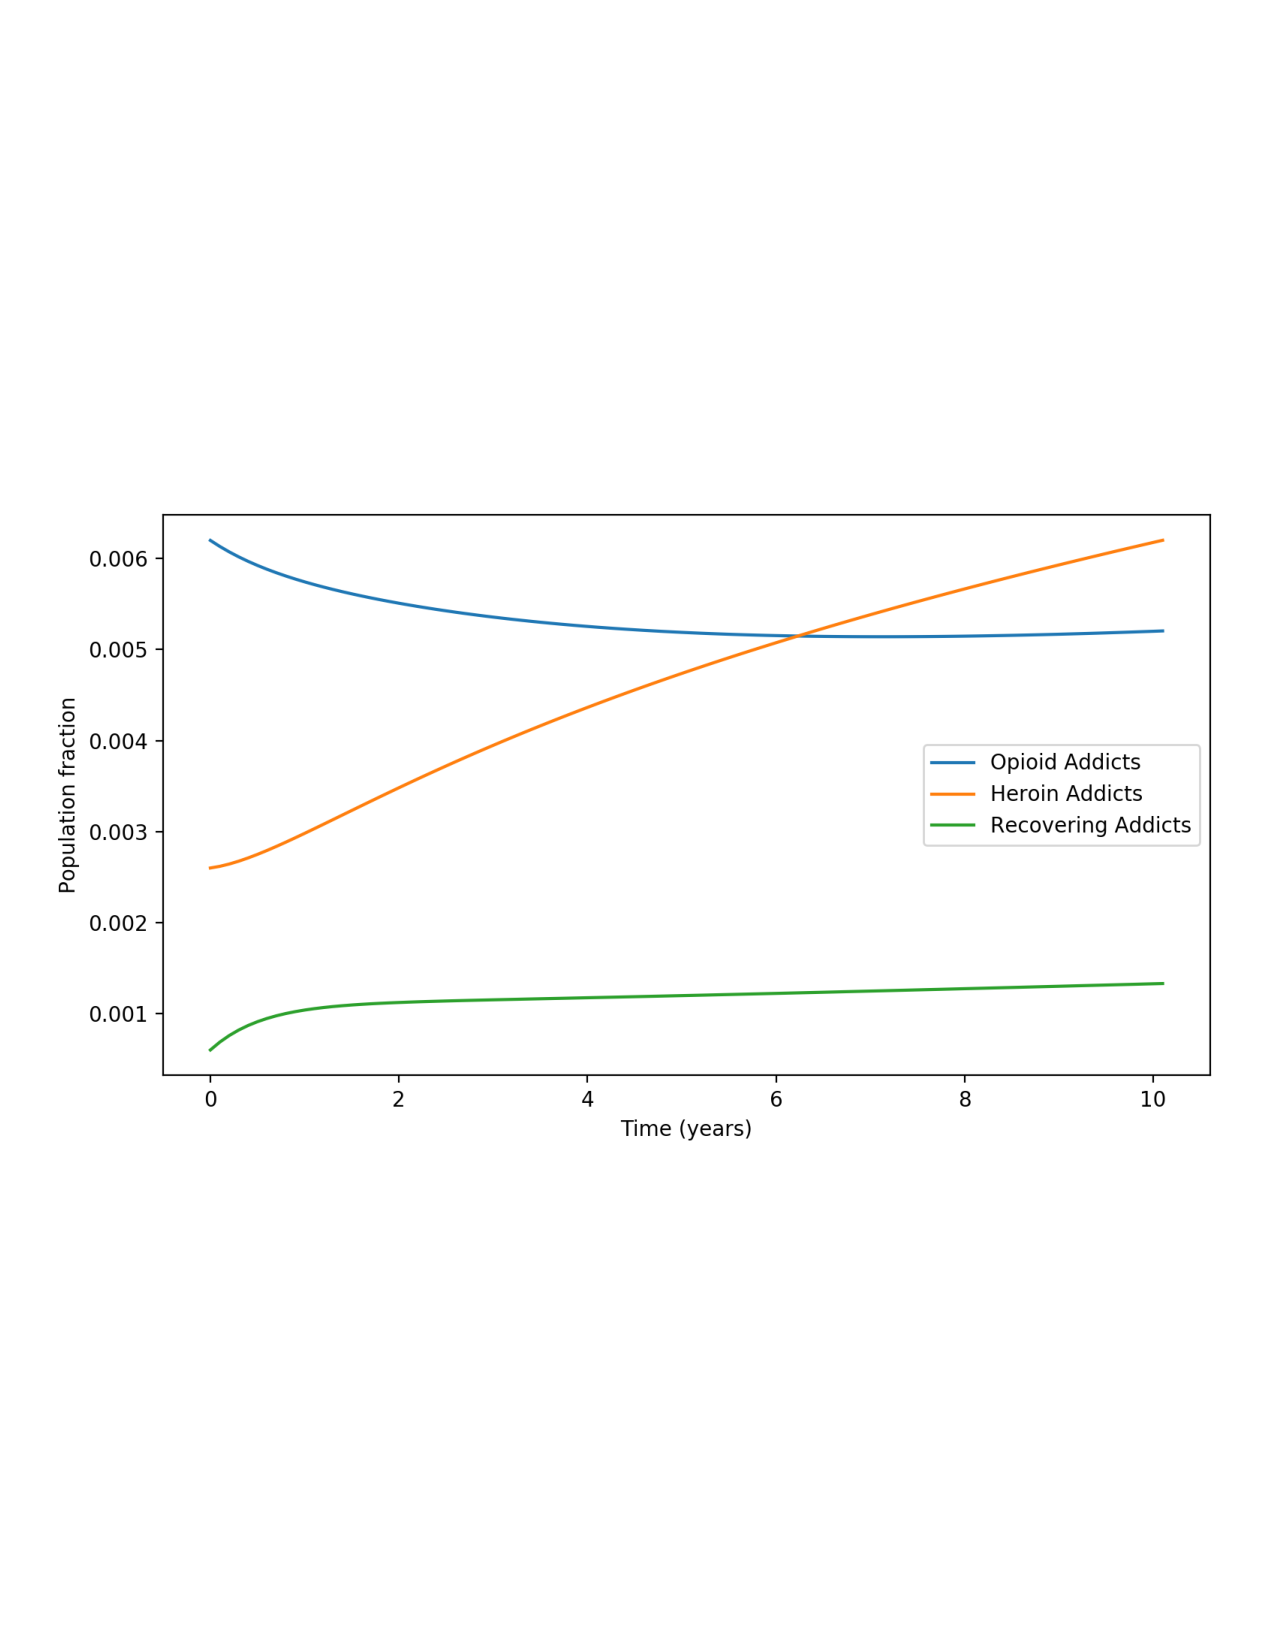
\includegraphics[width=.9\linewidth, height=0.27\textheight]{plot_remove_delta_separate}
\vspace{-.5cm}
\caption{Model without delta}
\end{minipage}
\end{figure}

\vspace{-1.4cm}


\begin{figure}[!htb]
\hspace{-.85cm}
\begin{minipage}{.6\textwidth}
\centering
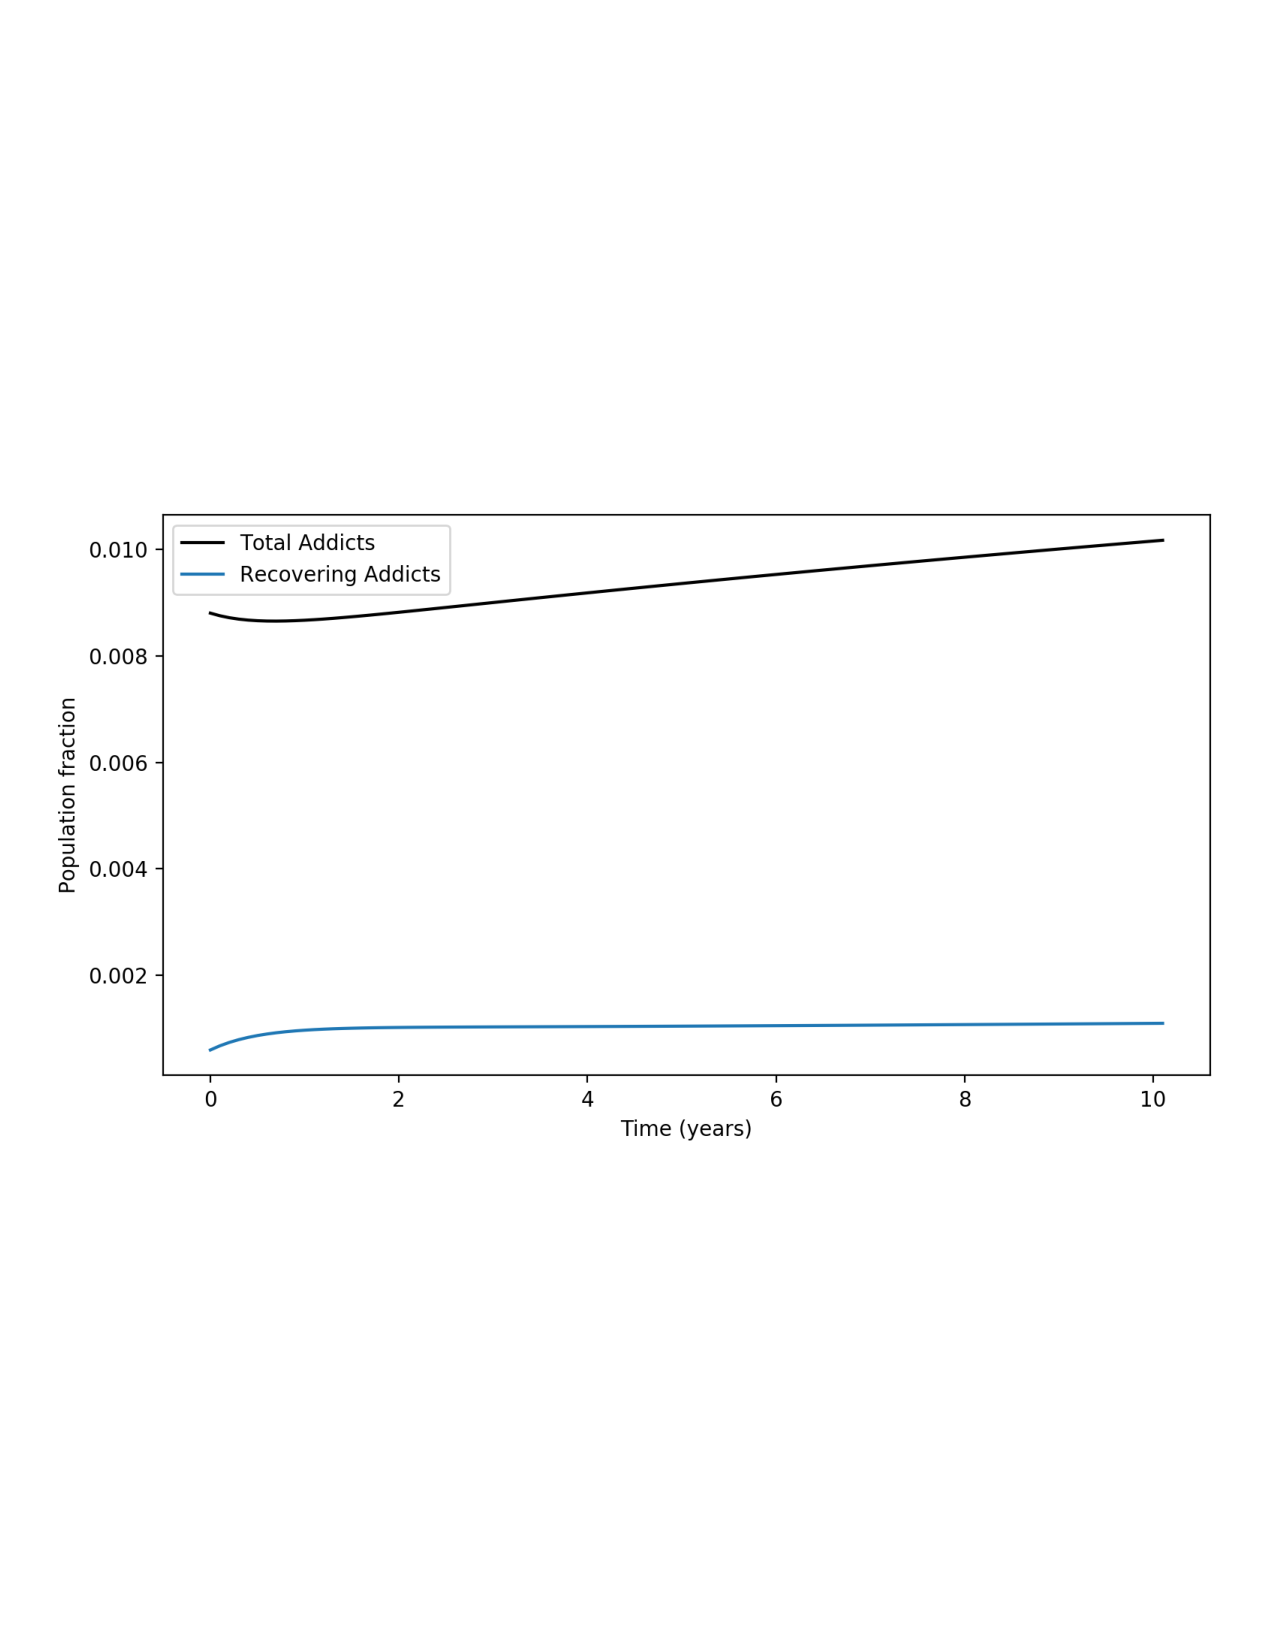
\includegraphics[width=.94\linewidth, height=0.28\textheight]{plot_with_delta_total}
\caption{Model including delta}
\end{minipage}
\hspace{-1.2cm}
\begin{minipage}{.6\textwidth}
\vspace{.8cm}
\centering
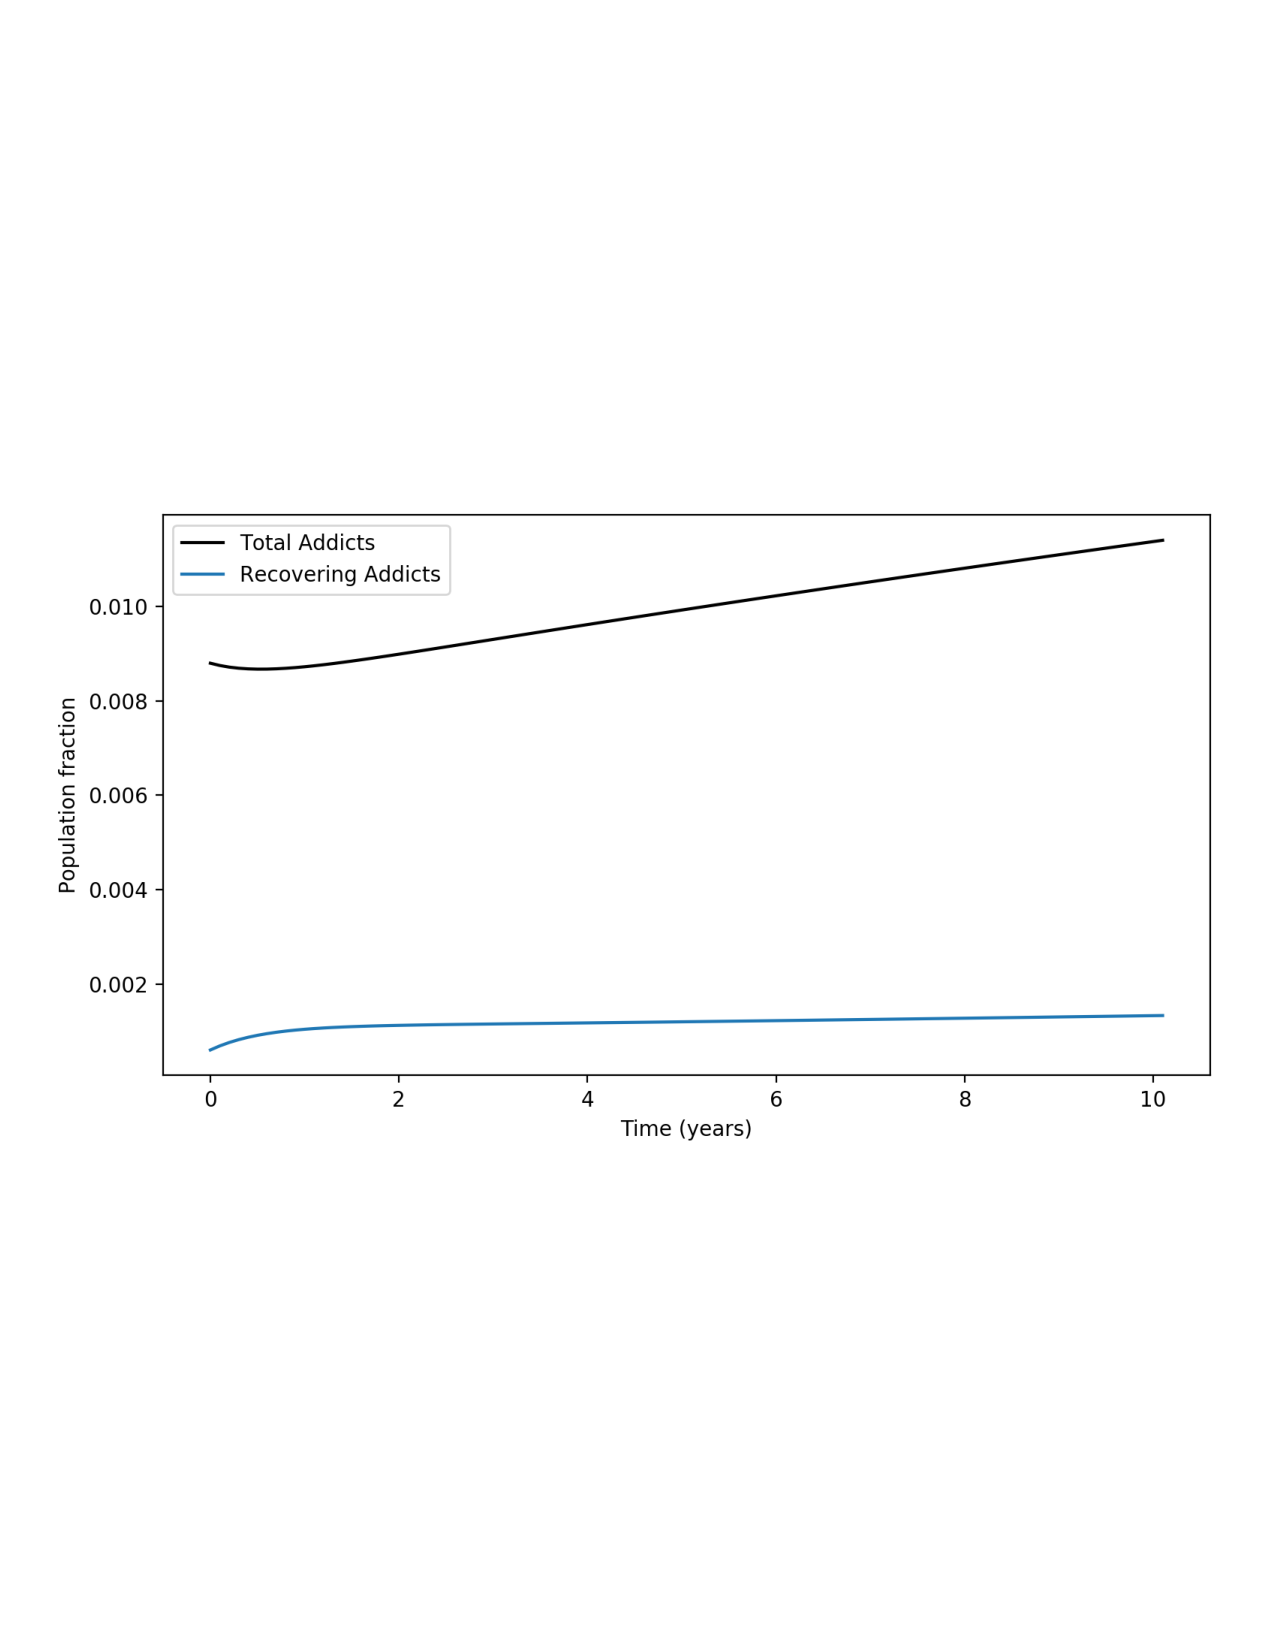
\includegraphics[width=.91\linewidth, height=0.266\textheight]{plot_remove_delta_total}
\caption{Model without delta}
\end{minipage}
\end{figure}






\pagebreak











\begin{figure}[!htb]


\hspace{-.7cm}
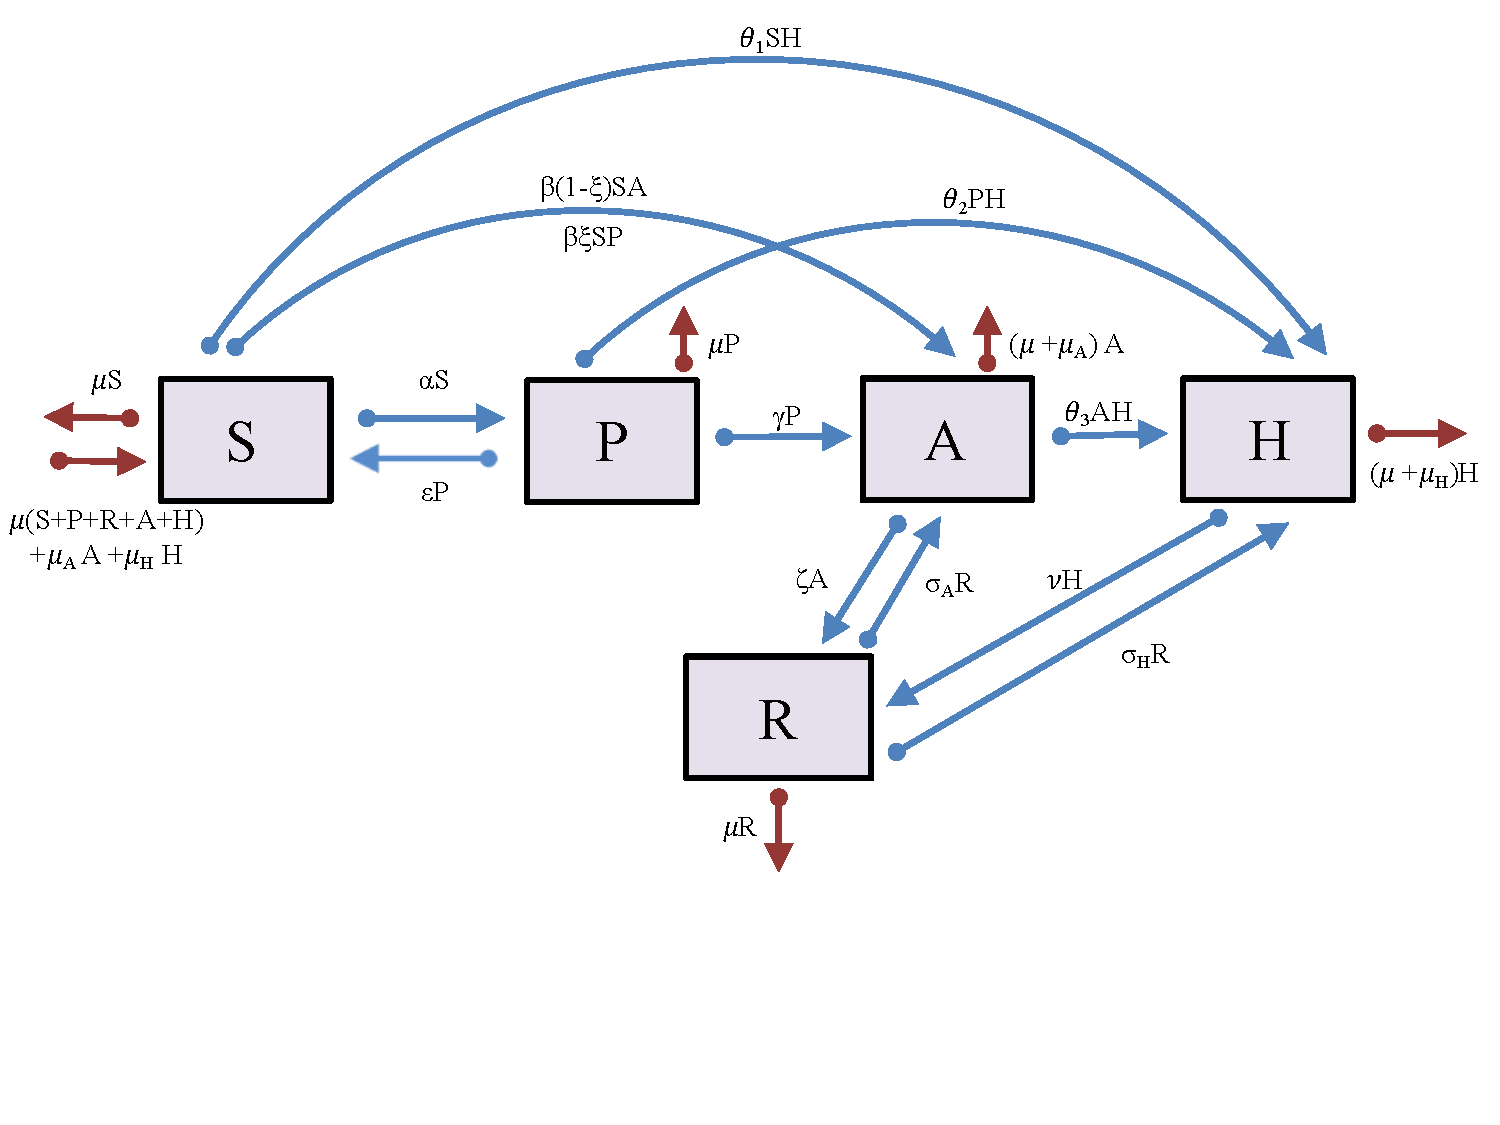
\includegraphics[width=1.1\linewidth, height=0.4\textheight]{heroin_schematic_without_delta_old_design}
\caption{Old schematic design}



\vspace{2cm}
\hspace{.8cm}
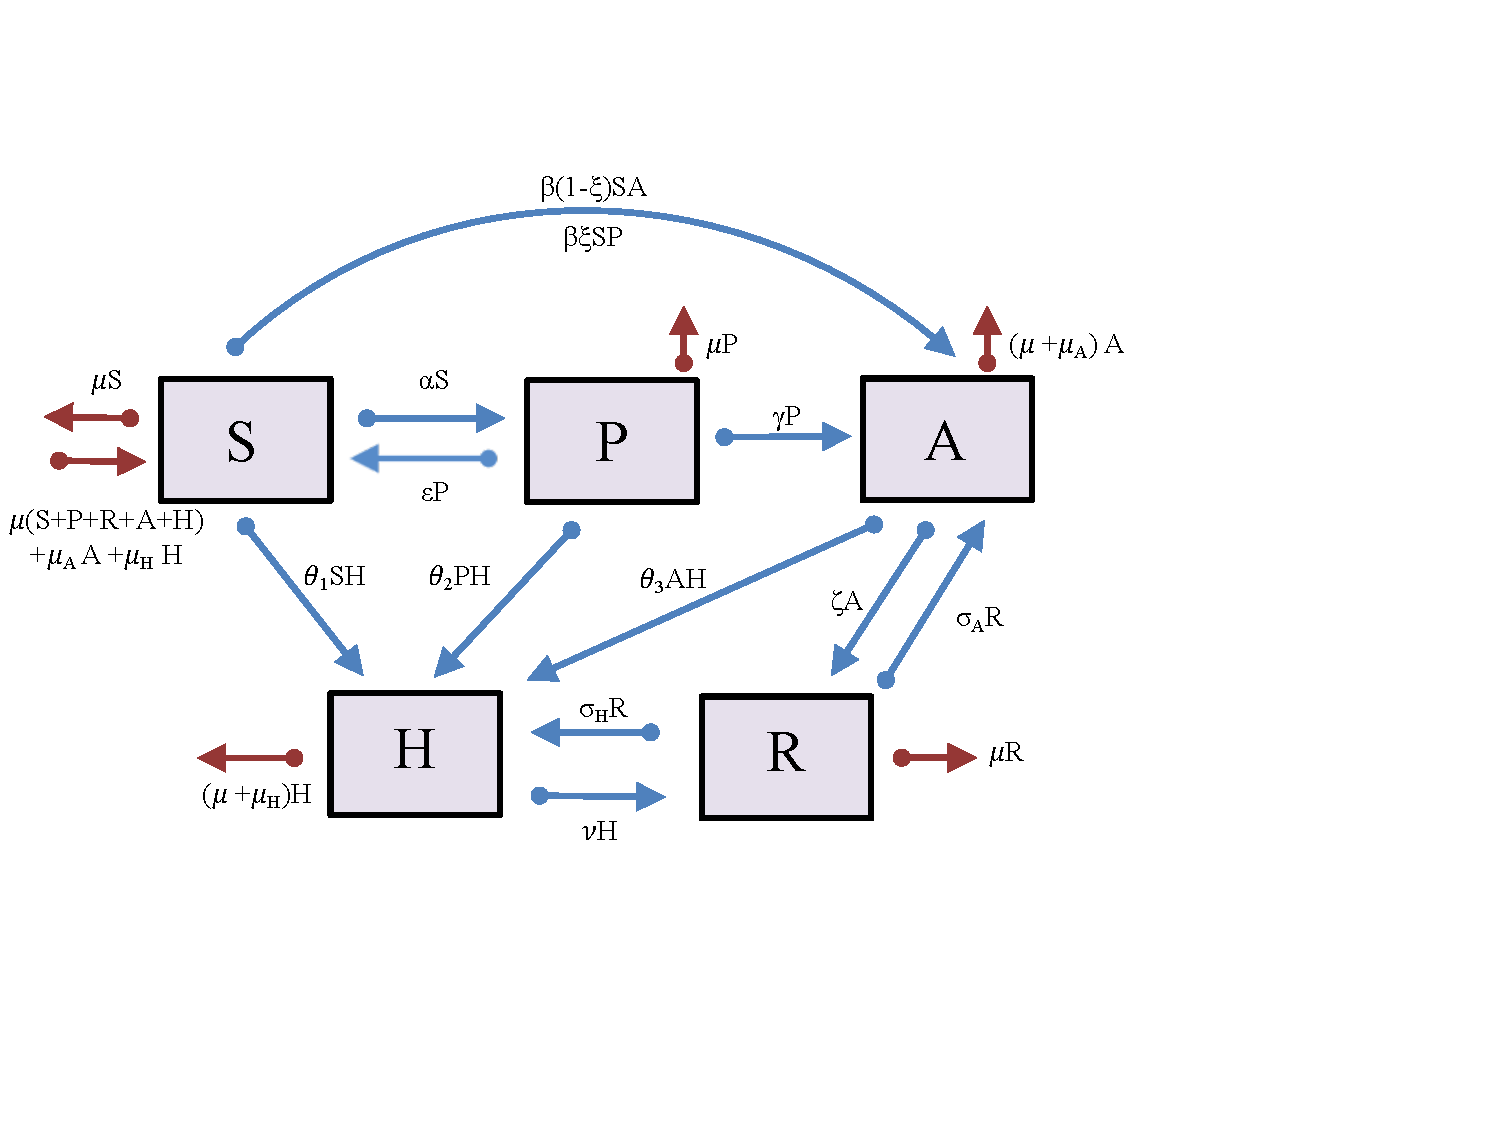
\includegraphics[width=0.9\linewidth, height=0.3\textheight]{heroin_schematic_without_delta_new_design}
\caption{New schematic design}

\end{figure}


\newpage


{[1]} Data Dashboard: https://www.tn.gov/health/health-program-areas/pdo/pdo/data-dashboard.html
\\
{[2]} PDO report: \\
https://www.tn.gov/content/dam/tn/health/documents/pdo/PDO\_2018\_Report\_02.06.18.pdf
{[3]} TN Mental Health and Substance Abuse Services: \\
 https://www.tn.gov/content/dam/tn/mentalhealth/documents/DPRF\_BH\_county\_ \\
 region\_service\_data \_book\_9-2017\_FINAL.pdf \\
{[4]} NSDUH for TN: https://www.samhsa.gov/data/report/2015-2016-nsduh-state-specific-tables \\
{[5]} CDC's Opioid Overdose Indicator Support Toolkit: https://pep-c.rti.org/HERO/KB/Documents\\/CDCs\%20Opioid\%20Overdose\%20Indicator\%20Support\%20Toolkit.pdf \\
{[6]} TN Department of Health: https://www.tn.gov/health/health-program-areas/statistics/health-data/death-statistics.html \\
{[7]} US Census Bureau:  https://www.census.gov/data/datasets/2017/demo/popest/state-total.html{\#}par{\_}textimage{\_}500989927
\\ \\

(Knox County has treatment admissions for 2014-2016 for prescription opioids, but not for heroin [3]. Can get heroin overdose deaths from [1] for Knox County, and opioid overdose deaths, but not parsed out with prescription opioid or fentanyl.) 









\bibliography{HeroinModel}

 \end{document}
